\documentclass[a4paper, oneside, 11pt]{article}
\pagestyle{plain}

% \setlength{\parindent}{6pt}
% \usepackage[skip=12pt]{parskip}

\usepackage[english]{babel}
\usepackage[margin=1.1in]{geometry}
\PassOptionsToPackage{hyphens}{url}\usepackage{hyperref}
\usepackage{titlesec}
\titlespacing*{\section}{0pt}{15pt}{10pt}
\usepackage{graphicx}
\usepackage{wrapfig}
\usepackage{xcolor}
\usepackage{pagecolor}
\usepackage{lipsum}
\usepackage{amsmath}
\usepackage{amsfonts}
\usepackage{mathtools}
\usepackage{amsthm}
\usepackage{listings}
\usepackage{tabularx}
\usepackage{lipsum}
\usepackage{multicol}
\usepackage{indentfirst}
\usepackage{authblk}

% \definecolor{myblack}{RGB}{45, 42, 46}
% \definecolor{mywhite}{RGB}{252, 252, 250}

% \pagecolor{myblack}
% \color{mywhite}

\titleformat{\chapter}[display]
	{\normalfont\bfseries}{}{0pt}{\Huge}

\author{
	\small{Matthew Kenely} \\
	\small{\texttt{matthew.kenely.21@um.edu.mt}}
}

\date{}


\definecolor{codegreen}{rgb}{0,0.6,0}
\definecolor{codegray}{rgb}{0.5,0.5,0.5}
\definecolor{codepurple}{rgb}{0.58,0,0.82}
\definecolor{backcolour}{rgb}{0.98,0.98,0.98}

\lstdefinestyle{mystyle}{
	backgroundcolor=\color{white},
	commentstyle=\color{codegreen},
	keywordstyle=\color{magenta},
	numberstyle=\tiny\color{codegray},
	stringstyle=\color{codepurple},
	basicstyle=\ttfamily,
	breakatwhitespace=false,
	breaklines=true,
	captionpos=b,
	keepspaces=true,
	numbersep=5pt,
	showspaces=false,
	showstringspaces=false,
	showtabs=false,
	tabsize=2
}

\lstset{style=mystyle}



\titleformat{\chapter}[display]
  {\normalfont\bfseries}{}{0pt}{\Huge}

\usepackage{enumitem}
\newlist{worddefs}{description}{1}
\setlist[worddefs]{font=\sffamily\bfseries, labelindent=\parindent, leftmargin=6em, style=sameline}

\title{\textbf{ARI2201 Individual Assigned Practical Task} \\ Location Chronicles}

\begin{document}
\maketitle

\setlength{\columnsep}{1cm}

% \section{Supplementary Material}
% \begin{itemize}
%   \item  Artefact -- Source Code: \href{https://github.com/matthewkenely/ics2000}{\url{https://github.com/matthewkenely/ics2000}}
%   \item Artefact -- Live Site: \href{https://mkenely.com/ics2000/}{\url{https://mkenely.com/ics2000/}}
%   \item  Presentation: \href{https://drive.google.com/file/d/1TzZtqQNC5mssmYfW3KPul5OFlGCC5cKT/view?usp=sharing}{\url{https://drive.google.com/file/d/1TzZtqQNC5mssmYfW3KPul5OFlGCC5cKT/view?usp=sharing}}
% \end{itemize}

\begin{multicols*}{2}

  \begin{abstract}
    \textit{
      This project provides a brief overview of the concept of tailoring news articles to users' locations, a background of this area and highlights the lack of such a platform which tailors news to Maltese users on a per-village basis. To address this, a dataset of Maltese news articles exhaustive of the majority of Maltese villages was created, a Named Entity Recognition model capable of identifying where news articles took place was trained on this dataset, and a web application was developed using PHP, CSS, JS and Python so as to give users the ability to utilise this model to identify the locations in which news articles took place, as well the ability to filter the dataset of news articles based on their geographical location or whichever location they choose. The results and limitations of this project are discussed and future work in this area is proposed.
    }
  \end{abstract}


  \section{Introduction}
  % Brief introduction to the problem (emphasis on lack of maltese digitisation)

  The influx of data in recent years has contributed to the quality of news platforms significantly, with the provision of personalised news content based on users' locations and preferences becoming more accurate by the day. These platforms often focus on larger geographical regions such as countries or cities. For users in smaller regions such as Malta, however, there is a lack of localised news content that caters to their specific interests and preferences on a per-village basis.

  Malta has a unique landscape with distinct villages, each with its own local events, issues, and news. For users residing in Malta, having access to news articles that are specifically relevant to their local villages can greatly enhance their news consumption experience and keep them informed about happenings in their immediate surroundings.

  % Aim of this project
  The aim of this project is to develop a platform for Maltese users which facilitates the recognition of where news articles took place geographically, as well as the ability to filter a database of news articles based on geographical locations, either tailored to a user's location or to whichever village they select. This entails the creation of a Maltese news article dataset, as well as the training of a machine learning model on this dataset to recognise locations in news articles.

  % Explanation of NLP and NER
  The task of recognising locations in news articles is a Natural Language Processing (NLP) problem, and more specifically, a Named Entity Recognition (NER) problem. NLP is a field of artificial intelligence (a scientific field that studies the creation of machines capable of performing tasks which normally require human intelligence \cite{poole2010artificial}) that deals with the interaction between computers and human (natural) languages. NER is a subtask of NLP which deals with the identification of named entities (subjects of interest) in text, such as people, locations and organisations \cite{nadeau2007survey}. In this project, the task of the developed NER algorithm will be to identify locations (specifically, Maltese villages) in news articles so as to determine where they took place.

  % Requirements
  To successfully create this platform, the following tasks shall be carried out:
  \begin{enumerate}
    \item The creation of a \textbf{dataset} of news articles which take place in (and mention) Maltese villages.
    \item The training of a \textbf{Named Entity Recognition model} on this dataset, with the goal of it being able to recognise where previously unseen Maltese news articles took place.
    \item The development of a \textbf{web application} on which the following features will be hosted:
          \begin{itemize}
            \item An article location detector which utilises the trained model to identify locations in news articles provided by the user.
            \item A news article database lookup which allows the user to filter said articles in the created dataset based on where they took place in Malta, either tailored to their location (given their consent) or to whichever village they select.
          \end{itemize}
  \end{enumerate}


  \section{Background}
  % Related work
  In recent years, the tendency has been for people to consume news on online platforms \cite{bennett2008digital} \cite{ripolles2012beyond}, offering users a vast amount of news articles from various sources. One popular example of such a platform is \href{https://news.google.com/}{Google News}, a news aggregator that collects headlines and snippets from news sources worldwide, allowing users to access a wide range of news articles on different topics. One key feature of Google News relevant to this project is its ability to tailor news articles to users' locations. This feature works well when it comes to filtering news articles on a per-country basis (including Malta), and while the option to filter on a per-village basis is available, it is not refined, with Google News often returning any articles which took place in Malta rather than in a specific village.

  \begin{center}
    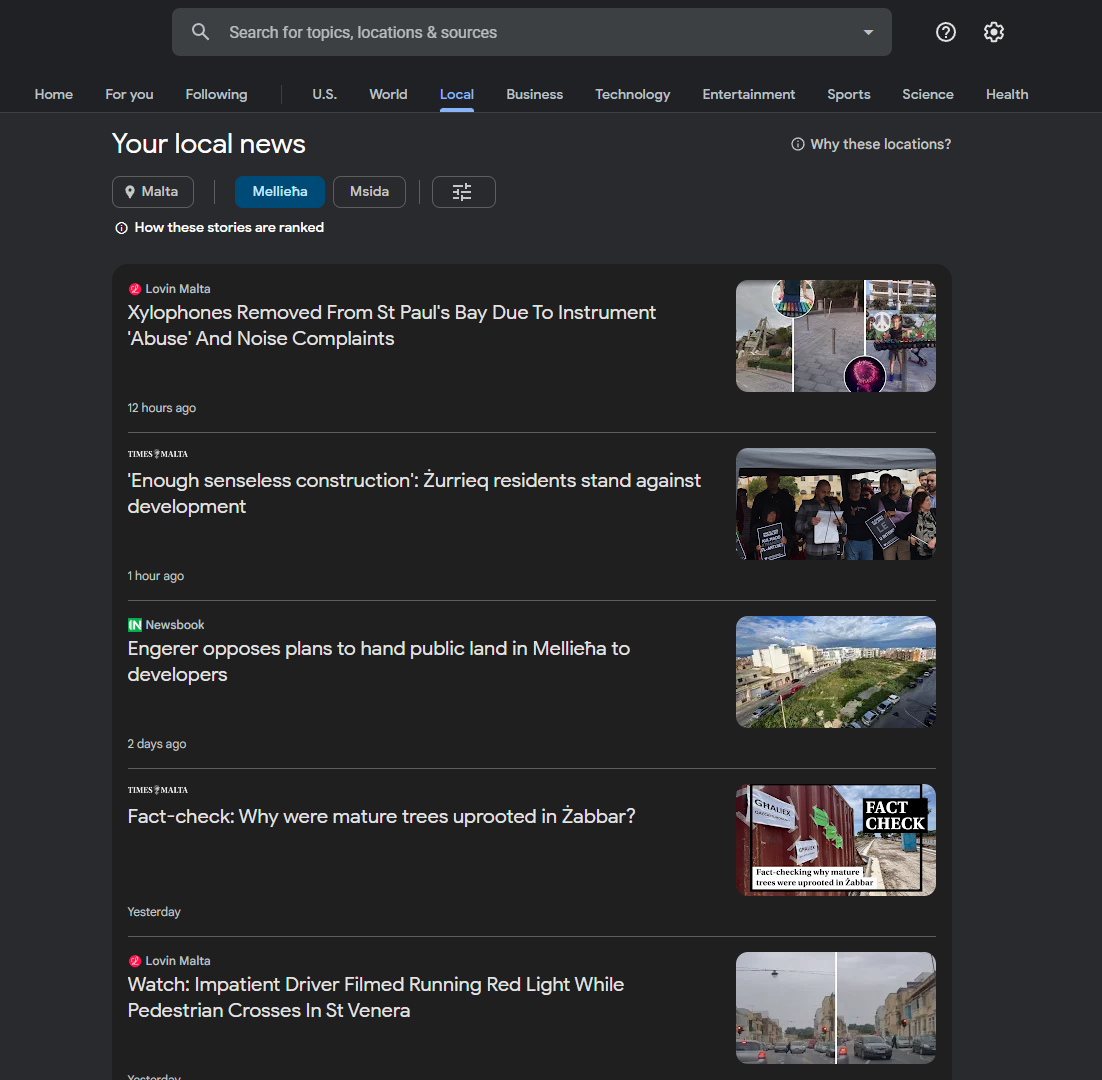
\includegraphics[width=0.5\textwidth]{./figures/googlenewsmellieha.png} \\
    Figure 1: Google News filtering by village (Mellieha) displaying articles which took place in St. Paul's Bay, Żurrieq and Żabbar
  \end{center}


  BBC News also offers this feature to a limited extent in its \href{https://www.bbc.com/news/world}{World} section, allowing users to filter news articles on a per-continent basis. However, this feature is not available for smaller geographical regions, and as such, cannot tailor news to a user based on the country they live in, let alone the specific city/village.


  \section{Methodology}
  \subsection{Dataset}
  \textit{All source files for work related to this section can be found in the} \verb|docs/data| \textit{directory}

  \medskip

  To create a dataset of Maltese news articles, I created algorithms (found in \verb|scraper.ipynb|) which scrape news articles in the \href{https://newsbook.com.mt/}{Newsbook}, \href{https://www.maltatoday.com.mt/}{MaltaToday} and \href{https://www.independent.com.mt/}{The Malta Independent} English local archives. After cleaning this data (specifically removing duplicates and normalising date formats) in Google Sheets I was able to scrape the following content of 14,177 news articles: URL, title, date, article text. This was followed by a filtering process to only include articles which mention the names of Maltese villages (found in \verb|villages.txt|) in their text, as well as the start and end index of these villages within the text (this is required to train the NER model), resulting in a dataset of 5151 articles The code for this filtering process can be found in \verb|location_extractor.ipynb|. A final pass through of the dataset was carried out to get the URL of each article's corresponding image (if any) and add it to the dataset (this was done in \verb|scraper.ipynb|).

  \subsection{Model}
  \textit{All source files for work related to this section can be found in the} \verb|docs/data| \textit{directory}

  \medskip

  The Named Entity Recognition model for this project was trained using the \href{}{spaCy} library in Python. spaCy is an open-source library for NLP written in Python, which provides a wide range of NLP tools and features, including the ability to train custom NER models.

  I used the blank English model provided by spaCy as a base model (with the intention of creating a model targeted towards the recognition of the names of Maltese villages), and proceeded to train it on the \verb|location_articles_images| dataset, taking the news article text and corresponding village name indices and entity labels (scraped in the Dataset subsection) as inputs. The model was trained for 10 epochs, with a dropout rate of 0.3.

  The code used to train the model can be found in \verb|train_model.ipynb|. The model was saved in the \verb|model| directory.


  \subsection{Web Application}
  \textit{All source files for work related to this section can be found in the} \verb|docs| \textit{directory}

  \medskip

  % Overview (mention mobile responsiveness, OpenStreetMap, etc.)
  The web application for this project was developed using PHP, CSS, JavaScript and Python. The application must be hosted (this can be done locally using open-source software such as \href{https://www.apachefriends.org/}{XAMPP}).

  The primary functions of the application (article location detection and database lookup) are implemented using forms which make POST requests to the server, pass POST parameters to external PHP scripts which run their corresponding Python scripts and return the results of the NER model and database filter respectively.

  The application is mobile responsive, allowing users to access it from whichever device they prefer.

  The application makes use of the \href{https://www.openstreetmap.org/}{OpenStreetMap} API to display a map of Malta on the home page, as well find the coordinates of the villages identified by the Article Location Detector and subsequently display said villages on the map. The Navigator Geolocation API is used on the the News page to ask the user for permission to access their location, which, if provided, is used to automatically filter the news articles in the database based on the village the user is currently in.

  \subsubsection{Home Page}
  The home page contains a form (called the Article Location Detector) which allows the user to input a news article URL, which is then passed to the NER model to attempt to identify the Maltese village in which the article took place.

  \subsubsection{News Page}
  The news page contains a form (called the Database Lookup) which allows the user to either provide their current location or select a village manually, which is then passed to a python script which filters the \verb|location_articles_images.csv| dataset, and retrieves news articles which mention that village. I opted for this approach in the case of database retrieval as while news articles may not have necessarily taken place in a user's chosen location, the fact that they mention said location may indicate that the article is of interest to individuals from that location regardless. The articles are then displayed on a grid of cards, each containing the article title, date, image (if any), and a link to the original article. The cards are sorted by date, with the most recent articles appearing first.


  \section{Results}
  \subsection{Dataset}
  % Mention good coverage of all villages but may be biased towards more active ones such as Valletta
  \begin{center}
    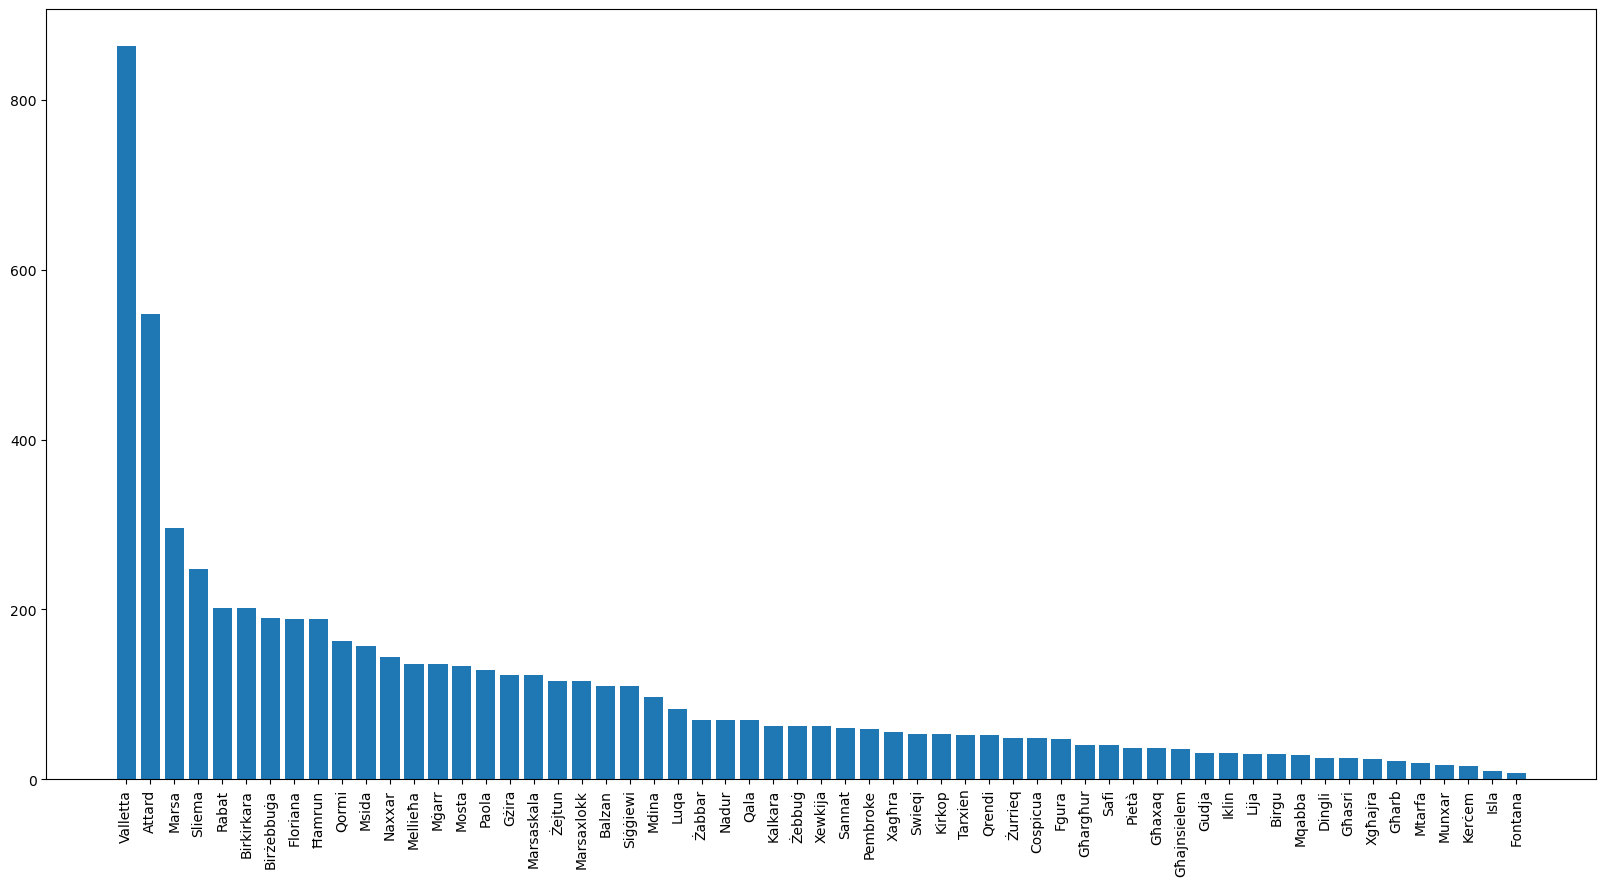
\includegraphics[width=0.5\textwidth]{./figures/villagefreq.png} \\
    Figure 2: Frequency of villages in the dataset
  \end{center}

  \begin{center}
    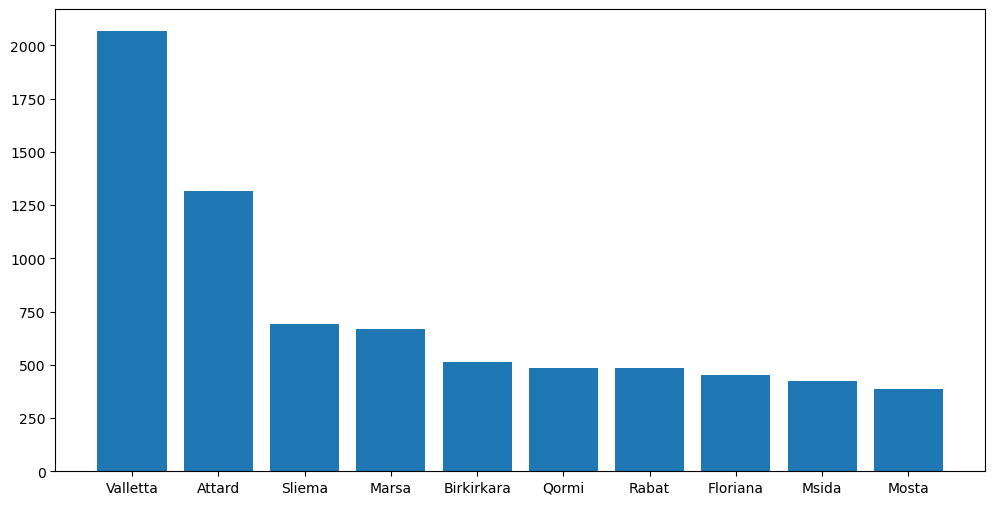
\includegraphics[width=0.5\textwidth]{./figures/villagefreqtop10.png} \\
    Figure 3: Top 10 most frequently appearing villages
  \end{center}

  As can be observed in the above figures, the dataset contains news article which occurred in almost all Maltese villages, with most articles taking place in Valletta. This is to be expected given that Valletta is the capital city of Malta and is a very active village.

  The dataset is not undersampled in any way and hence is biased towards more active villages. This is not an issue when it comes to the training of an NER model as the linguistic contexts in which the names of villages occur are the same regardless of the popularity of the village, and hence the model will be able to recognise the names of villages (and generalise the contexts in which they appear) regardless of how often they occur in the dataset. Users will simply be shown less articles for less active villages when using the database filter feature.


  \subsection{Model}
  % Do some testing on the model (e.g. show some examples of articles it got right and wrong)
  \begin{center}
    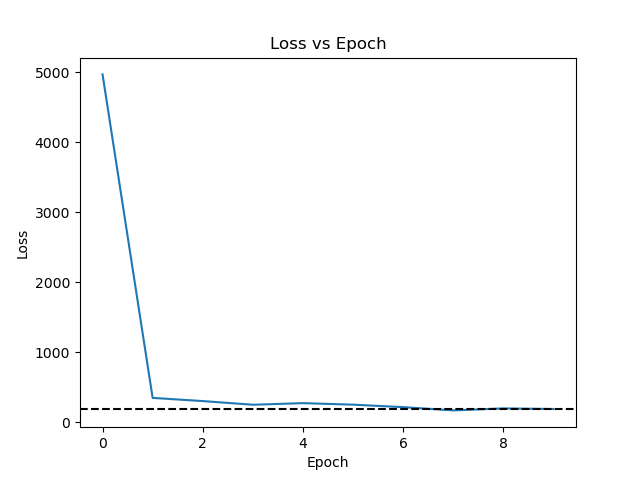
\includegraphics[width=0.5\textwidth]{./figures/nerloss.png} \\
    Figure 4: Loss of the NER model over 10 epochs
  \end{center}

  The following are series of test news articles which were passed to the NER model, where they took place, and the village which the model identified as the location (if any) in which the article took place.

  \begin{enumerate}
    \item \href{https://newsbook.com.mt/en/mellieha-councillor-urges-mps-to-block-development-in-natura-2000-site/}{Mellieha councillor urges MPs to block development in Natura 2000 site}
          \begin{itemize}
            \item[$\rightarrow$] Took place in: \textbf{Mellieha}
            \item[$\rightarrow$] Predicted location: \textbf{Mellieha}
          \end{itemize}
          \item\href{https://newsbook.com.mt/en/a-sea-of-people-join-puttinu-cares-in-17km-charity-walk/}{`A sea of people' join Puttinu Cares in 17km charity walk}
          \begin{itemize}
            \item[$\rightarrow$] Took place in: (Ambiguous)
            \item[$\rightarrow$] Predicted location: \textbf{Mosta}
          \end{itemize}
          \item\href{https://newsbook.com.mt/en/zurrieq-residents-last-stand-against-plans-to-zone-nigret-farmland-for-apartments/}{Żurrieq residents’ last stand against plans to zone Nigret farmland for apartments}
          \begin{itemize}
            \item[$\rightarrow$] Took place in: \textbf{Żurrieq}
            \item[$\rightarrow$] Predicted location: \textbf{Żurrieq}
          \end{itemize}

          \item\href{https://timesofmalta.com/articles/view/pothole-luck-400-drivers-claim-compensation-bad-roads-two-years.1032416}{Pothole luck: 400 drivers claim compensation for bad roads in two years}
          \begin{itemize}
            \item[$\rightarrow$] Took place in: mainly \textbf{Siġġiewi}
            \item[$\rightarrow$] Predicted location: \textbf{Siġġiewi}
          \end{itemize}
  \end{enumerate}

  On the whole, the model performs well, correctly identifying the news artcile location in tests 1, 3 and 4.

  In test 2, the news article took place in multiple villages (Mellieha, Xemxija, St Paul’s Bay, Mosta, Lija, Birkirkara, Msida, Pieta and Floriana), though it can be argued that primary villages of interest are Mellieha and Floriana. The model is, however, unable to identify either of these as the location in which the article ``took place''.


  \subsection{Web Application}
  % Show screenshots of the web app
  \begin{center}
    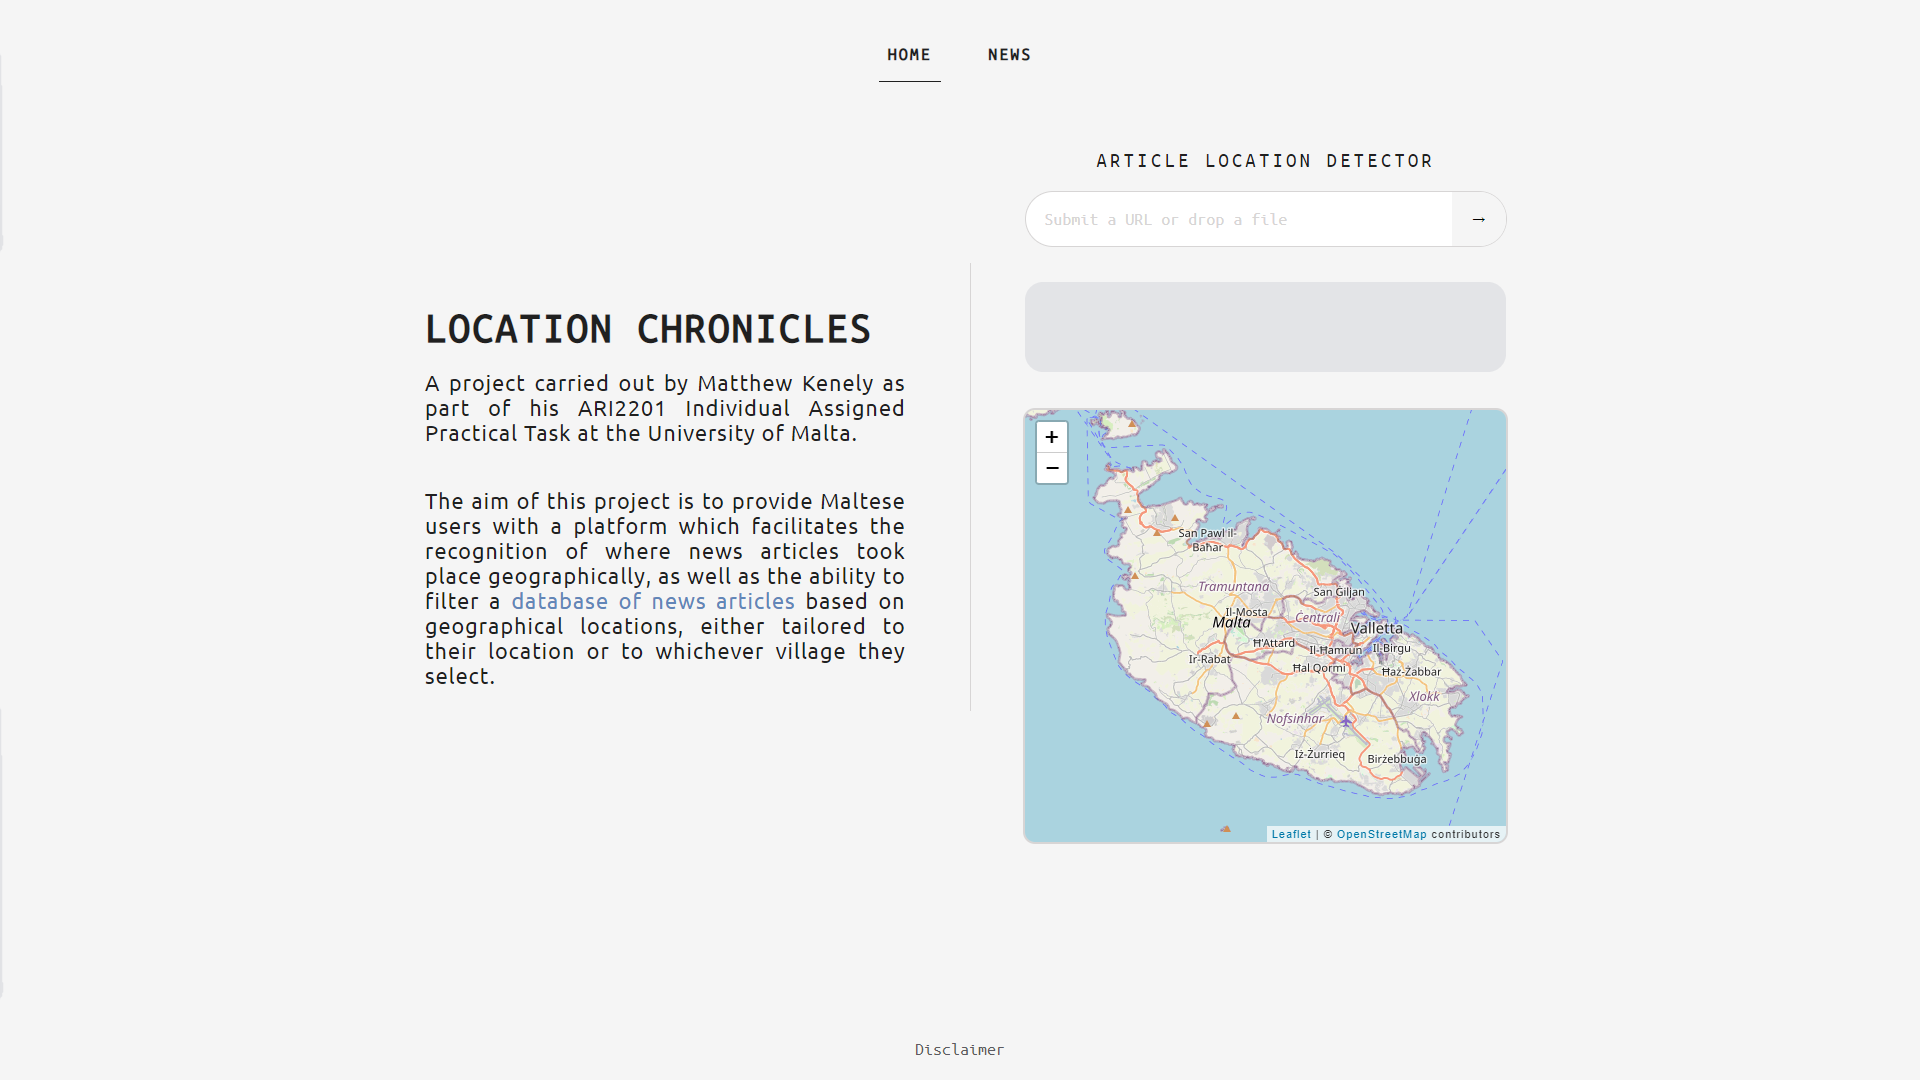
\includegraphics[width=0.5\textwidth]{./figures/homepage.png} \\
    Figure 5: Web application home page
  \end{center}

  \begin{center}
    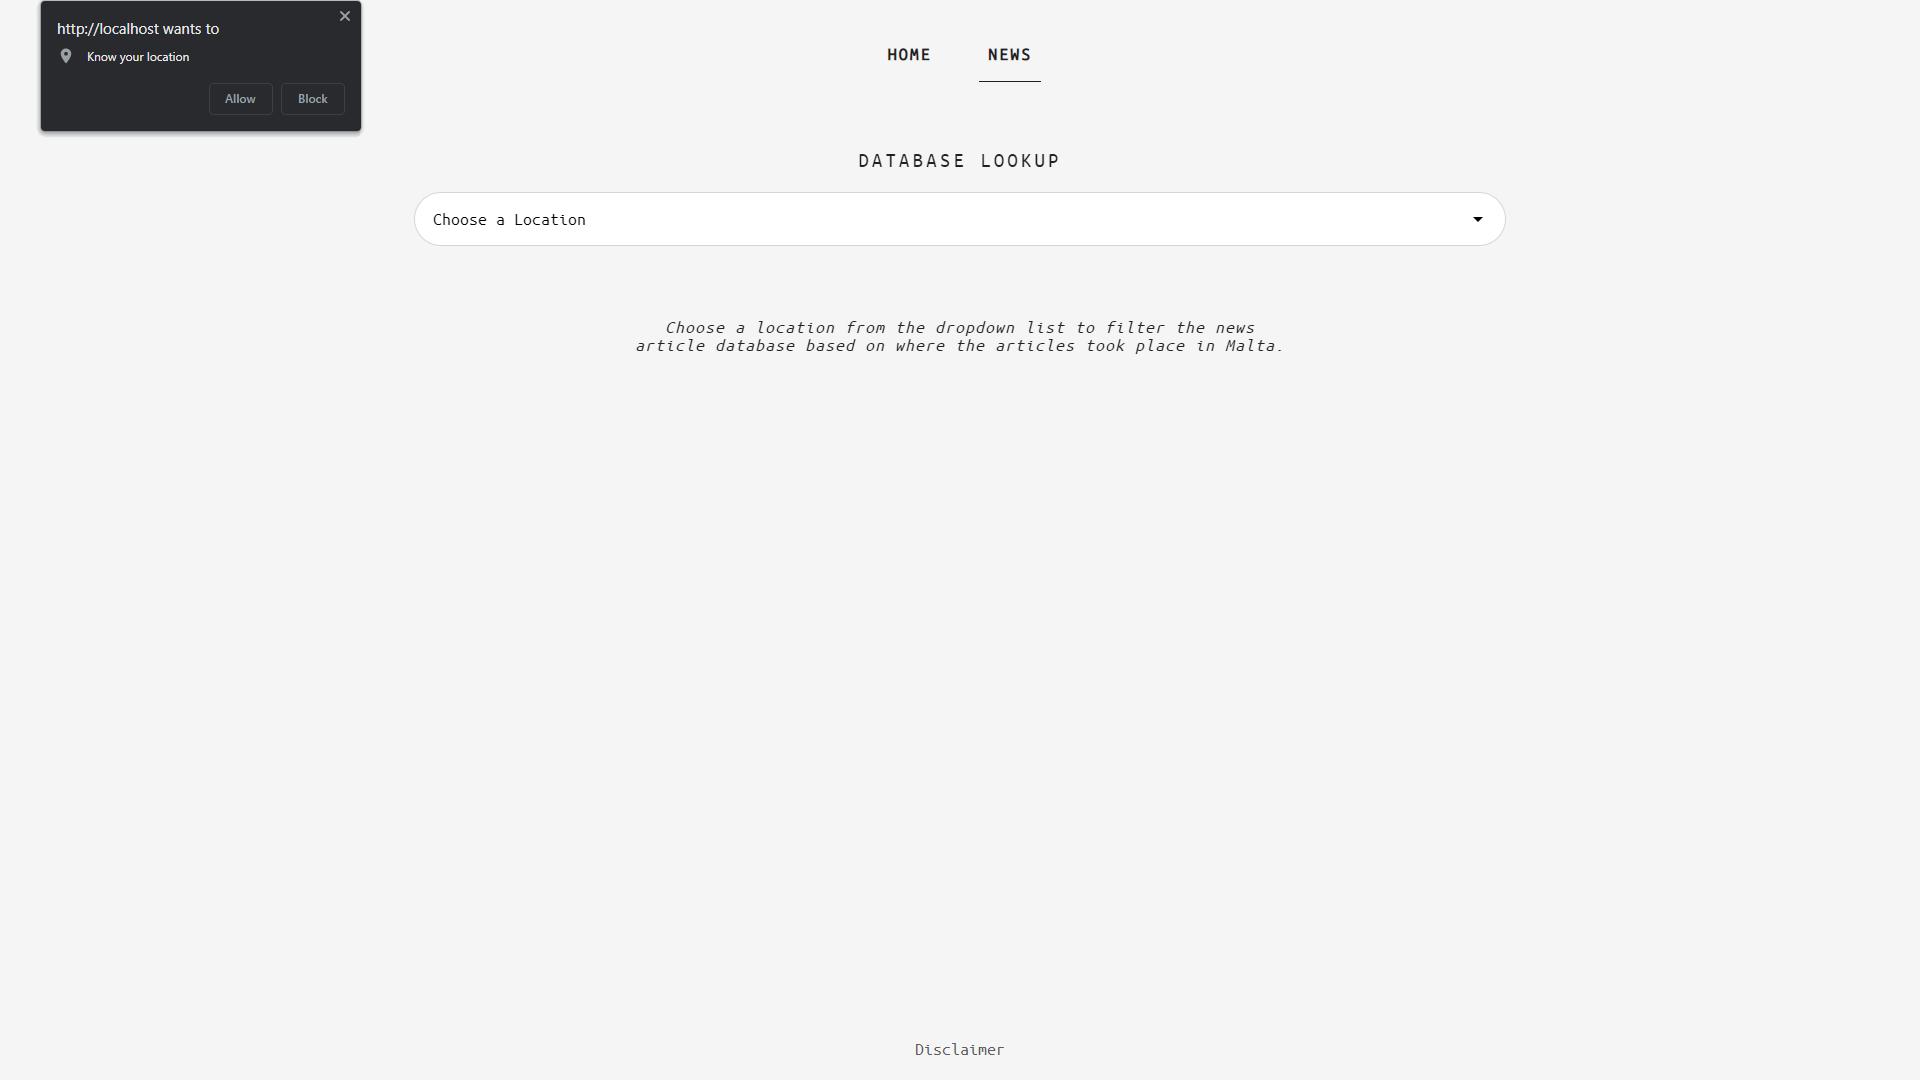
\includegraphics[width=0.5\textwidth]{./figures/newspagelocation.png} \\
    Figure 6: Web application news page (user is prompted for location)
  \end{center}

  \begin{center}
    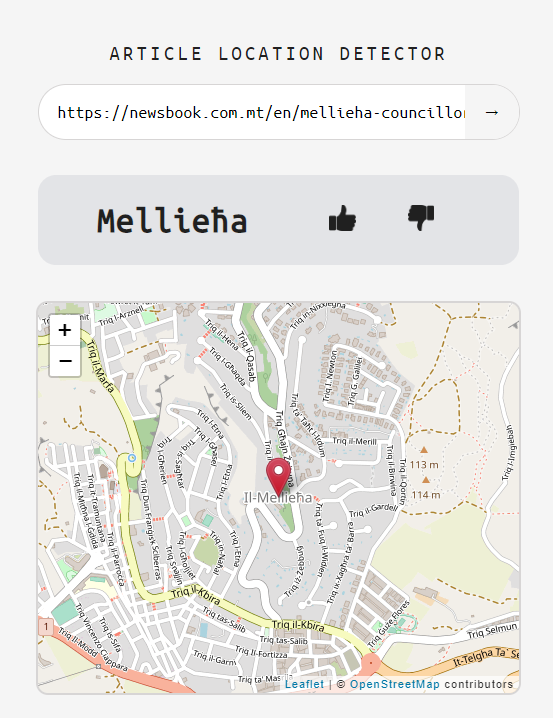
\includegraphics[width=0.5\textwidth]{./figures/locationdetector.png} \\
    Figure 7: Article location detector
  \end{center}

  \begin{center}
    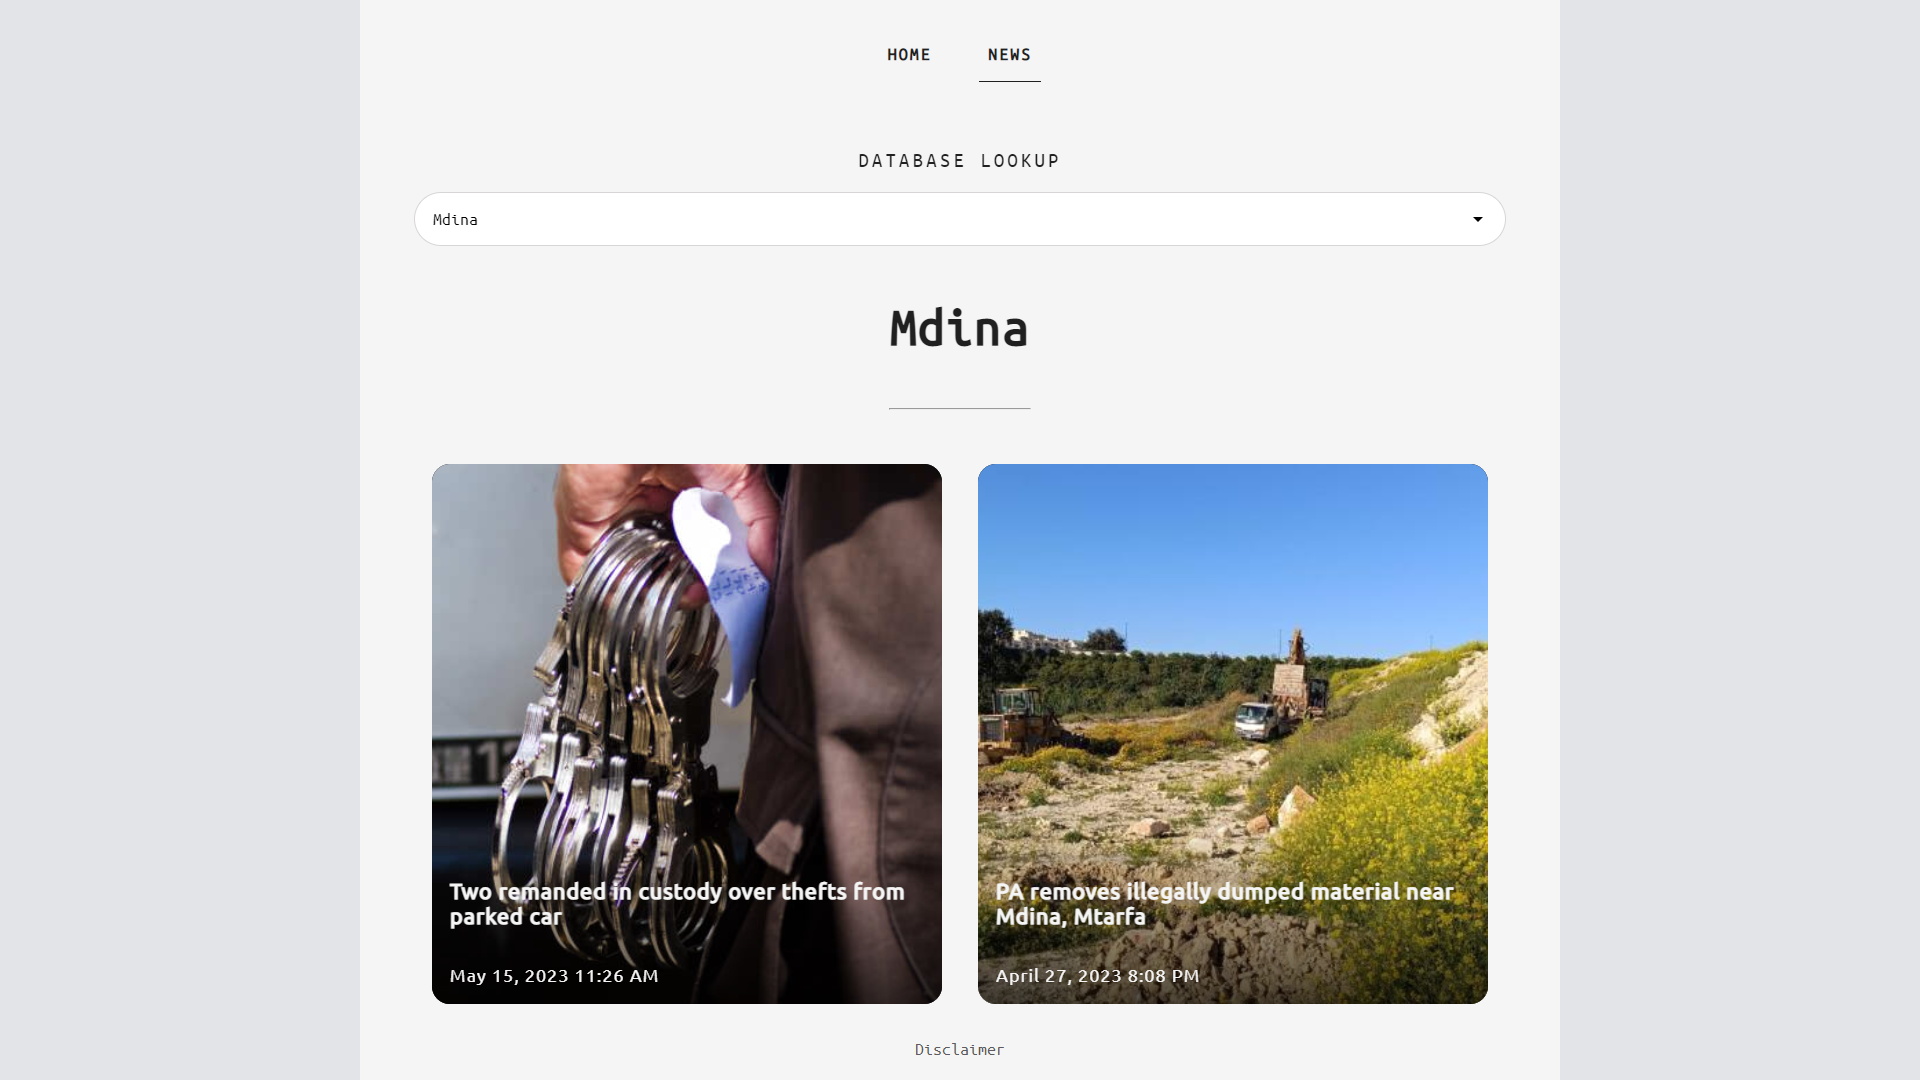
\includegraphics[width=0.5\textwidth]{./figures/newspagechoice.png} \\
    Figure 8: Web application news (user has chosen Mdina manually)
  \end{center}

  \begin{center}
    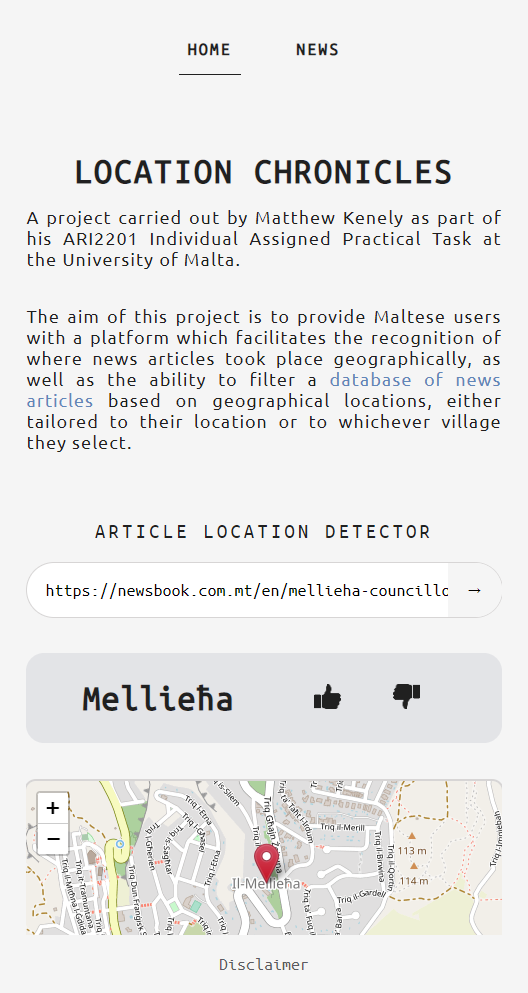
\includegraphics[width=0.5\textwidth]{./figures/mobilehome.png} \\
    Figure 9: Web application home page on mobile
  \end{center}

  \begin{center}
    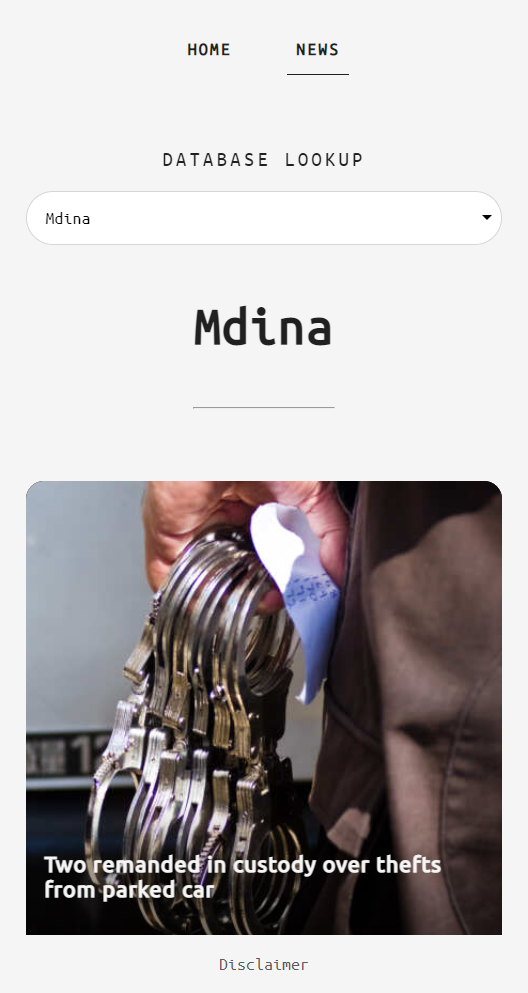
\includegraphics[width=0.5\textwidth]{./figures/mobilenews.png} \\
    Figure 10: Web application news page on mobile
  \end{center}

  As can be observed in the above figures, the web application is functioning as intended, with the Article Location Detector and Database Lookup forms successfully making POST requests to the server, calling their corresponding Python scripts and returning the results of the NER model and database filter respectively.

  In figure 5, the user is prompted to share their location. If they choose to do so, the application automatically filters the news articles in the database based on the village they are currently in. If they choose not to share their location, they are prompted to select a village manually, as shown in figure 7.

  The application is also fully mobile responsive, allowing users to access it from whichever device they prefer.



  \section{Challenges and Limitations}
  % Mention the lack of a Maltese NER model, and the lack of a Maltese NLP library

  % English articles only
  The dataset only contains English news articles. This is due to the fact that the NER model was trained on the English spaCy model, and hence is only able to recognise locations in English text. This is a limitation of the model, and can be addressed by training the model on a dataset of Maltese news articles, and using a Maltese NLP library such as

  % Village names containing multiple words (e.g. St. Paul's Bay)
  The model is unable to recognise village names which contain multiple words, such as St. Paul's Bay. This is due to the fact that the model was trained on a dataset of news articles which only contain single-word village names. This is a limitation of the model, and can be addressed by training the model on a dataset of news articles which contain multi-word village names, and labelling the village names in the text as such.

  % Articles which took place in multiple villages
  The model is unable to recognise the names of villages in news articles which took place in multiple villages. This is a limitation of the model, and can be addressed by training the model on a dataset which contains news articles which took place in multiple villages, and labelling the villages in which they took place as such.


  \section{Conclusion}
  % Summarise the project and its results
  In this project, I created a dataset of Maltese news articles, trained a Named Entity Recognition model on this dataset, and developed a web application which utilises this model to identify the locations in which news articles took place, as well as filter a database of news articles based on geographical locations.

  % Future work
  Future work on this project could include the following:
  \begin{itemize}
    \item Training the NER model on a dataset of Maltese news articles, and using a Maltese NLP library such
    \item Training the NER model on a dataset of news articles which contain multi-word village names, and labelling the village names in the text as such.
    \item Training the NER model on a dataset which contains news articles which took place in multiple villages, and labelling the villages in which they took place as such.
  \end{itemize}





  \newpage


  \Urlmuskip=0mu plus 1mu\relax
  \bibliographystyle{IEEEtran}
  \bibliography{refs}

\end{multicols*}


\end{document}